\subsection{Kiểm thử}

\subsubsection{Môi trường kiểm thử}
Các ca kiểm thử được thực hiện trên nhiều môi trường để đảm bảo tính tương thích của hệ thống:  
\begin{itemize}
	\item \textbf{Windows 11}: Phiên bản 23H2, CPU Intel(R) Core(TM) i5-1035G7 @ 1.20GHz, RAM 16GB.  
	\item \textbf{Ubuntu 22}: Cấu hình tương tự Windows (CPU Intel i5, RAM 16GB).  
	\item \textbf{Macbook Air M2}: CPU Apple Silicon M2, RAM 8GB.  
\end{itemize}
Trình duyệt sử dụng: Google Chrome (phiên bản mới nhất), chạy trên \texttt{localhost}.

\subsubsection{Phương pháp kiểm thử}
Mỗi test case bao gồm các thông tin: ID, tên, mô tả, kết quả mong đợi, module liên quan, và trạng thái chạy trên từng hệ điều hành.  
Kết quả được phân loại:  
\begin{itemize}
	\item \textbf{Pass}: Kết quả thực tế khớp với mong đợi (các cột OS được tick).  
	\item \textbf{Fail}: Kết quả thực tế khác mong đợi hoặc không chạy được (các cột OS không tick).  
\end{itemize}

\subsubsection{Kết quả kiểm thử theo module}
\begin{itemize}
	\item \textbf{Booking Module}  
	% \begin{center}
	% 	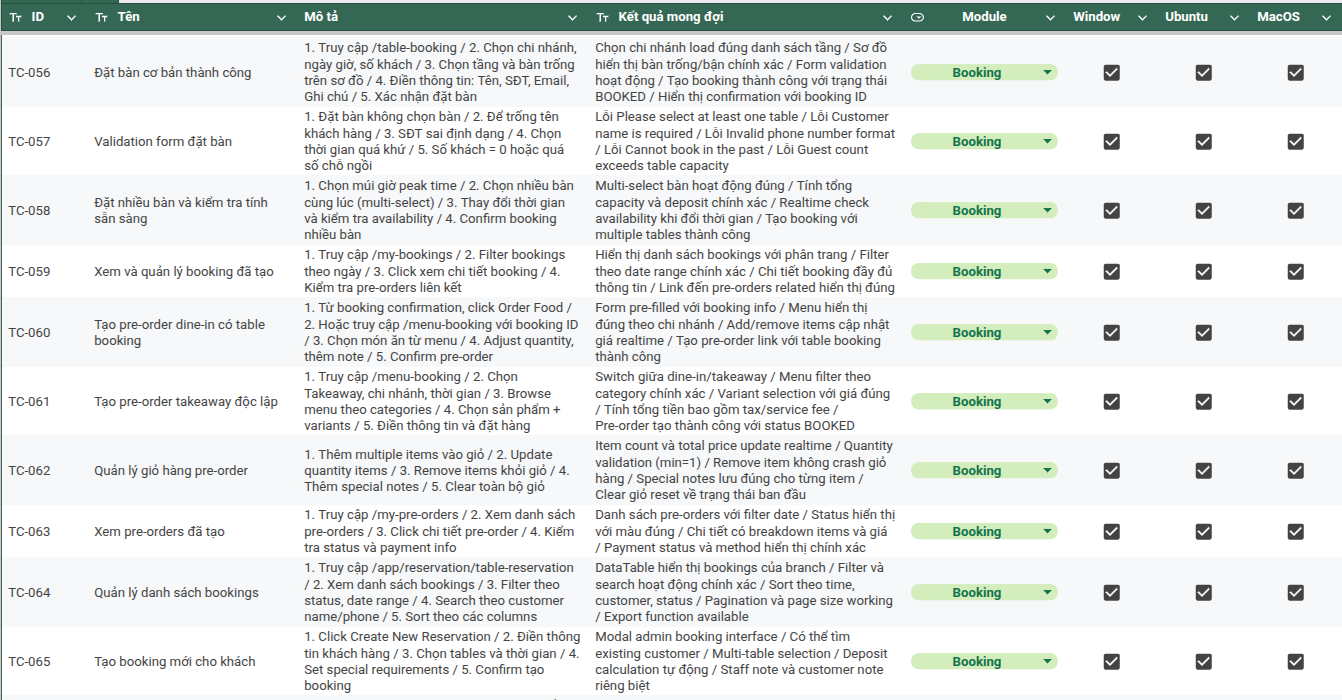
\includegraphics[width=14cm]{Images/hienthuc/test_booking.png}
	% \end{center}
    \begin{figure}[H]
        \centering
        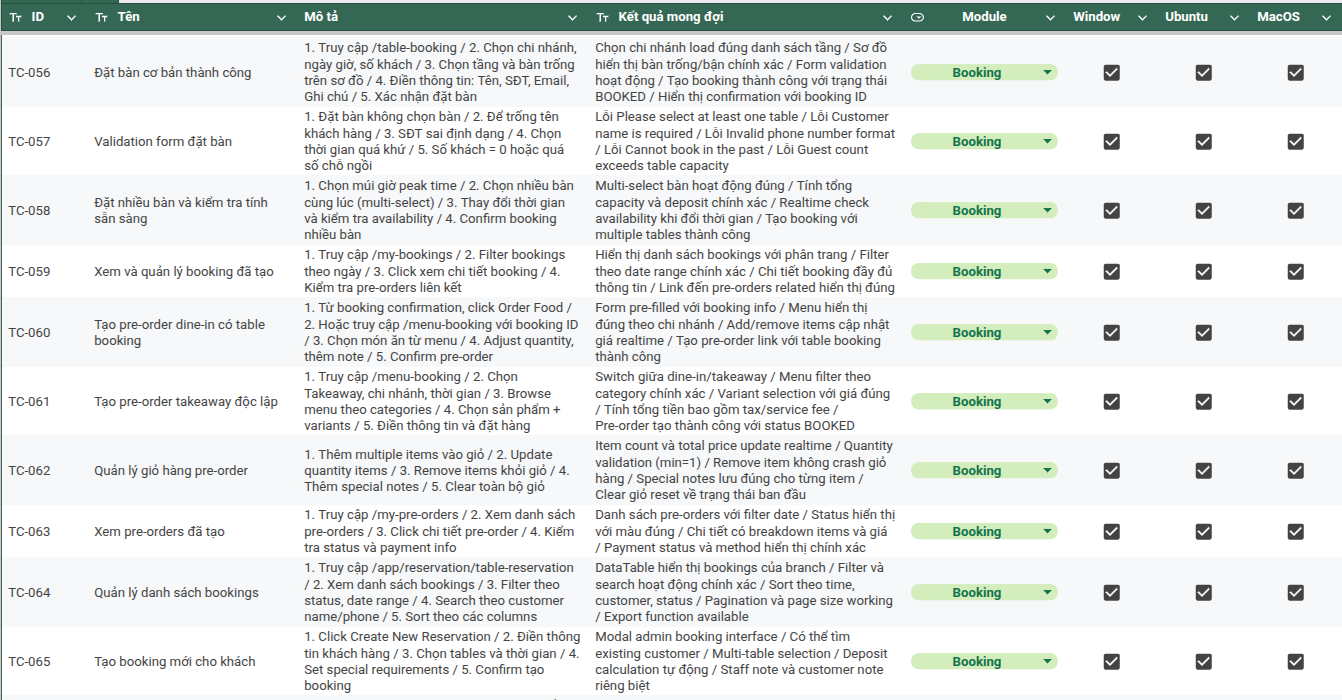
\includegraphics[width=14cm]{Images/hienthuc/test_booking.png}
		\vspace{0.5cm}
        \caption{Kết quả kiểm thử Booking Module}
		\label{fig:booking}
    \end{figure}
	Các ca kiểm thử về đặt bàn, quản lý booking, pre-order đều \textbf{Pass} trên cả ba môi trường.  
	Hệ thống đáp ứng đúng các yêu cầu: validation form, multi-table booking, quản lý giờ giữ bàn, và liên kết với pre-order.

	\item \textbf{Menu Module}  
	% \begin{center}
	% 	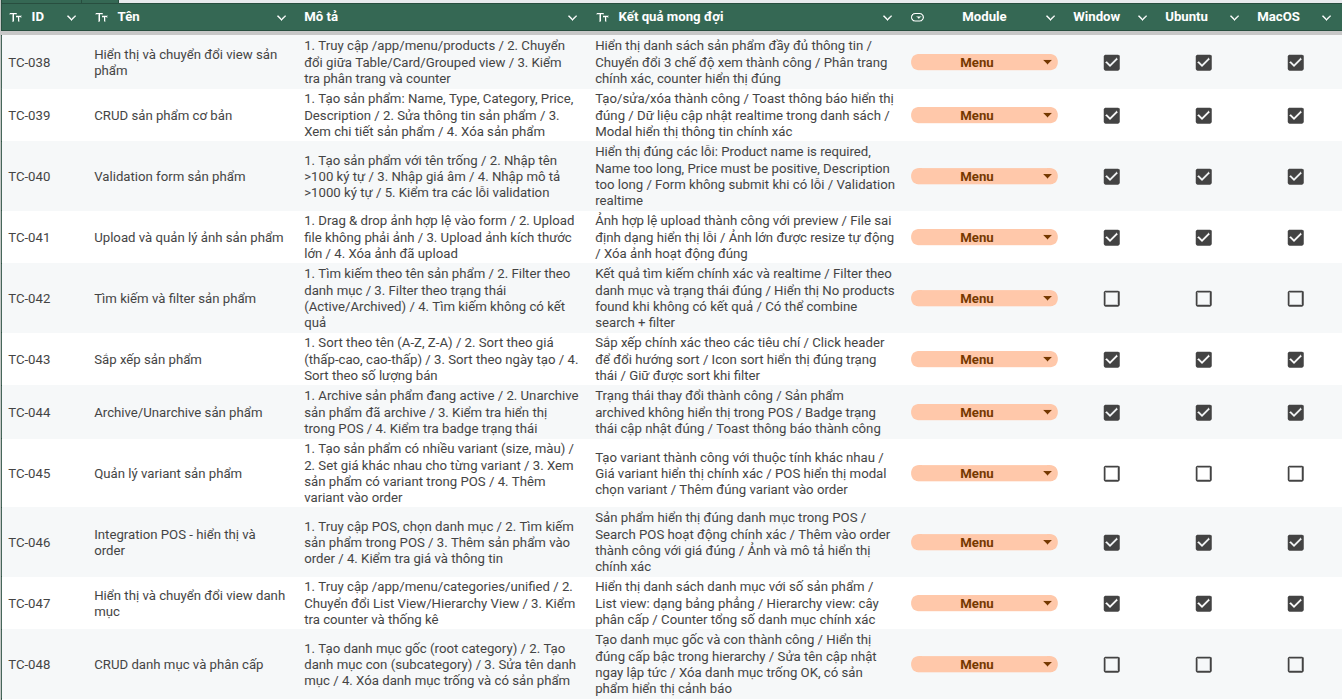
\includegraphics[width=14cm]{Images/hienthuc/test_menu.png}
	% \end{center}
    \begin{figure}[H]
        \centering
        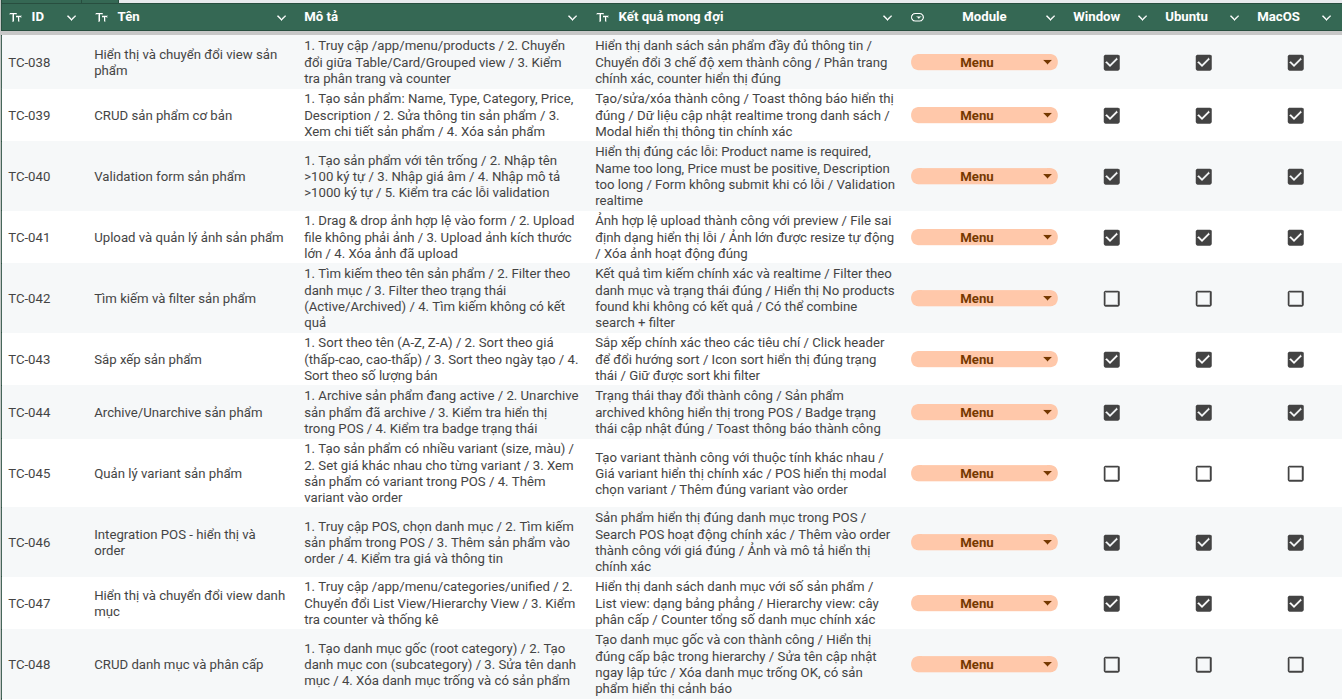
\includegraphics[width=14cm]{Images/hienthuc/test_menu.png}
		\vspace{0.5cm}
        \caption{Kết quả kiểm thử Menu Module}
		\label{fig:menu}
    \end{figure}
	Đa số test case \textbf{Pass}, như CRUD sản phẩm, upload ảnh, tìm kiếm/filter sản phẩm.  
	Tuy nhiên vẫn có một số \textbf{Fail}:  
	\begin{itemize}
		\item Chức năng \textbf{Delete Category} chưa hoạt động đúng.  
		\item Chức năng \textbf{Set Price cho Variant} không cập nhật được.  
	\end{itemize}
	Cần khắc phục để đảm bảo quản lý danh mục và giá sản phẩm hoàn chỉnh.

	\item \textbf{POS Module}  
	% \begin{center}
	% 	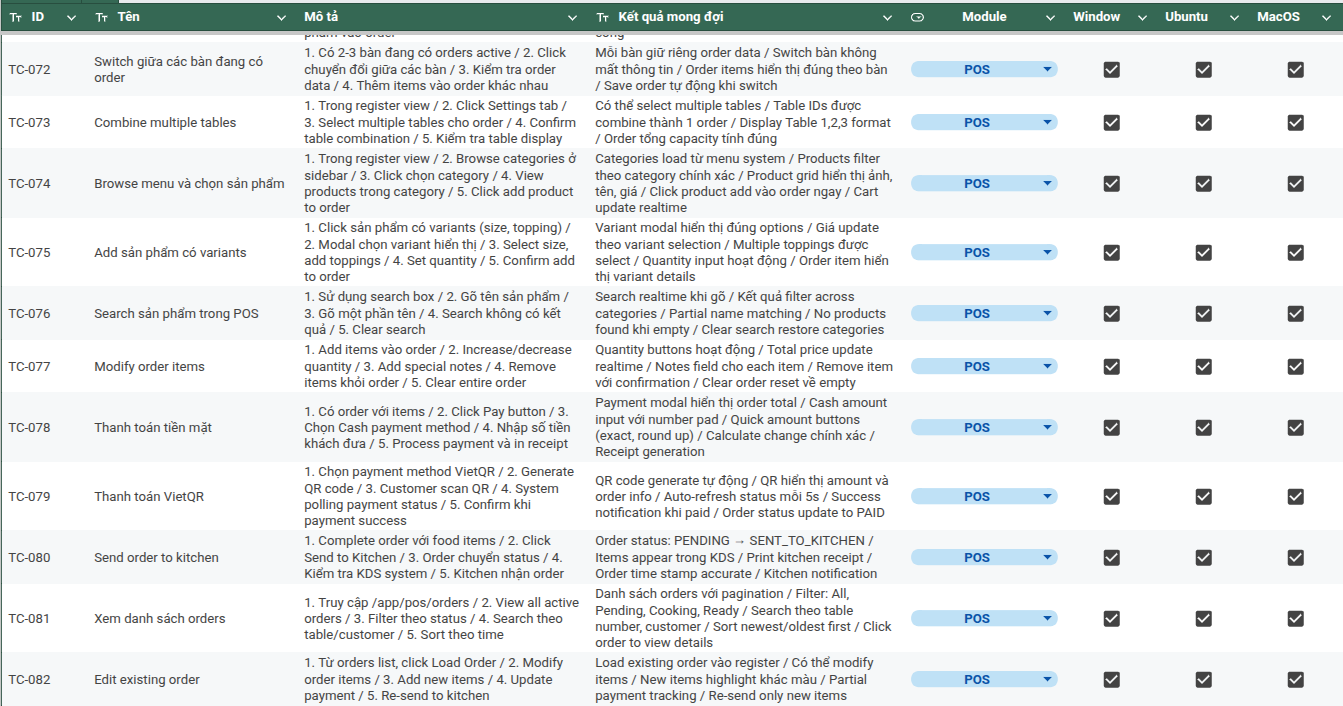
\includegraphics[width=14cm]{Images/hienthuc/test_pos.png}
	% \end{center}
    \begin{figure}[H]
        \centering
        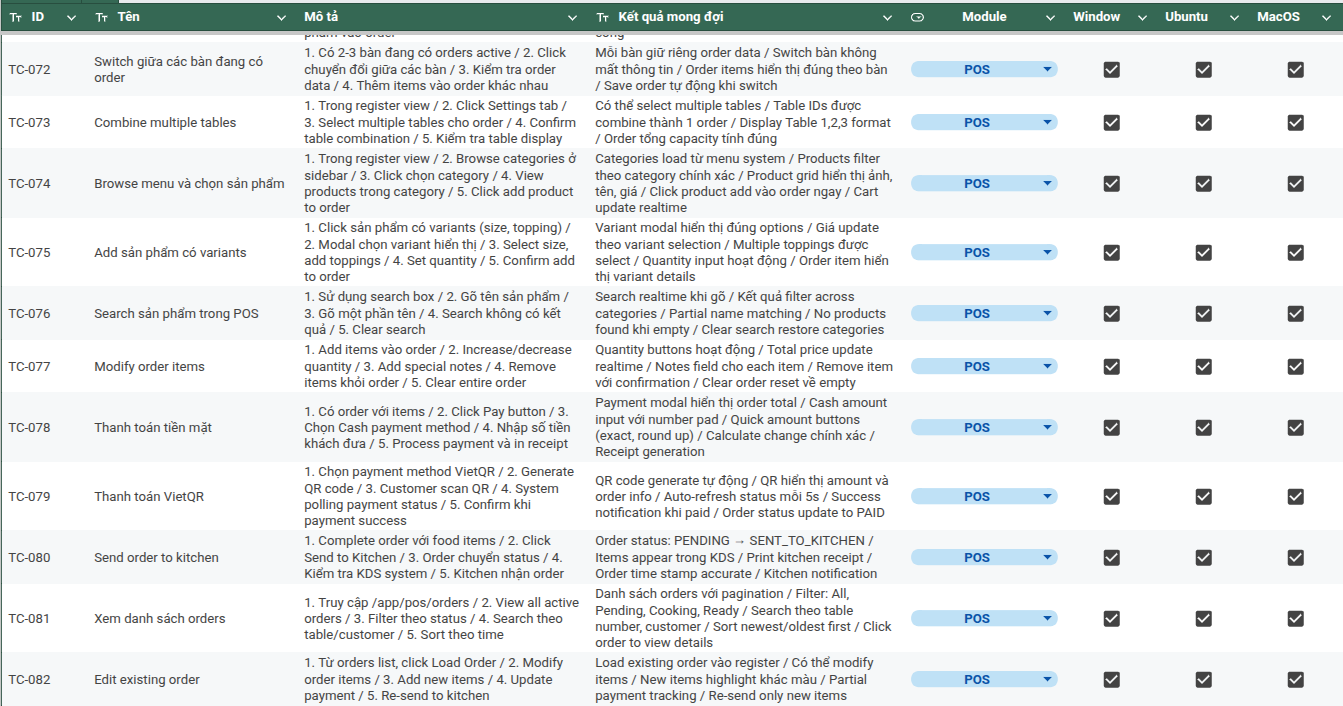
\includegraphics[width=14cm]{Images/hienthuc/test_pos.png}
		\vspace{0.5cm}
        \caption{Kết quả kiểm thử POS Module}
		\label{fig:pos}
    \end{figure}
	Các chức năng chính (thêm món, thanh toán tiền mặt/VietQR, gửi order đến bếp, sửa order) đều \textbf{Pass} trên các môi trường kiểm thử.  
	Điều này đảm bảo quy trình order tại POS diễn ra trơn tru.

	\item \textbf{Scheduling Module}  
	% \begin{center}
	% 	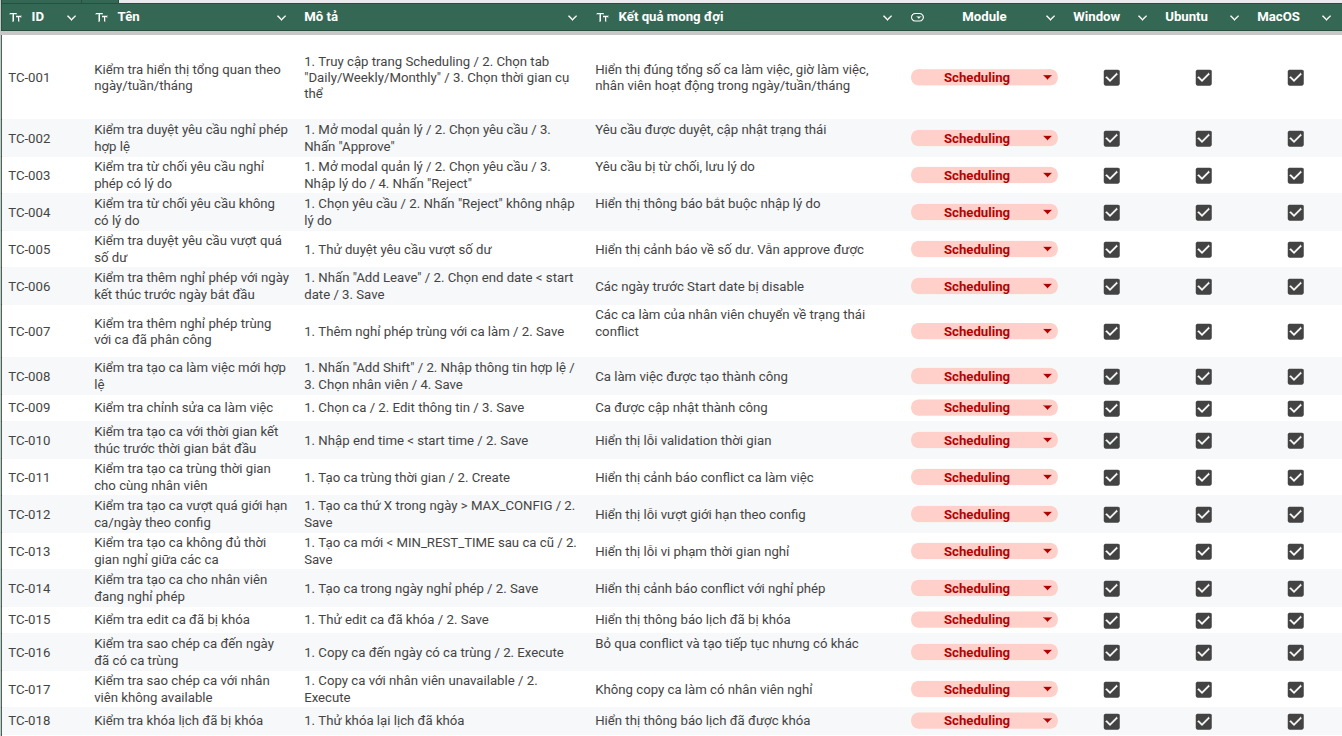
\includegraphics[width=14cm]{Images/hienthuc/test_schedule.png}
	% \end{center}
    \begin{figure}[H]
        \centering
        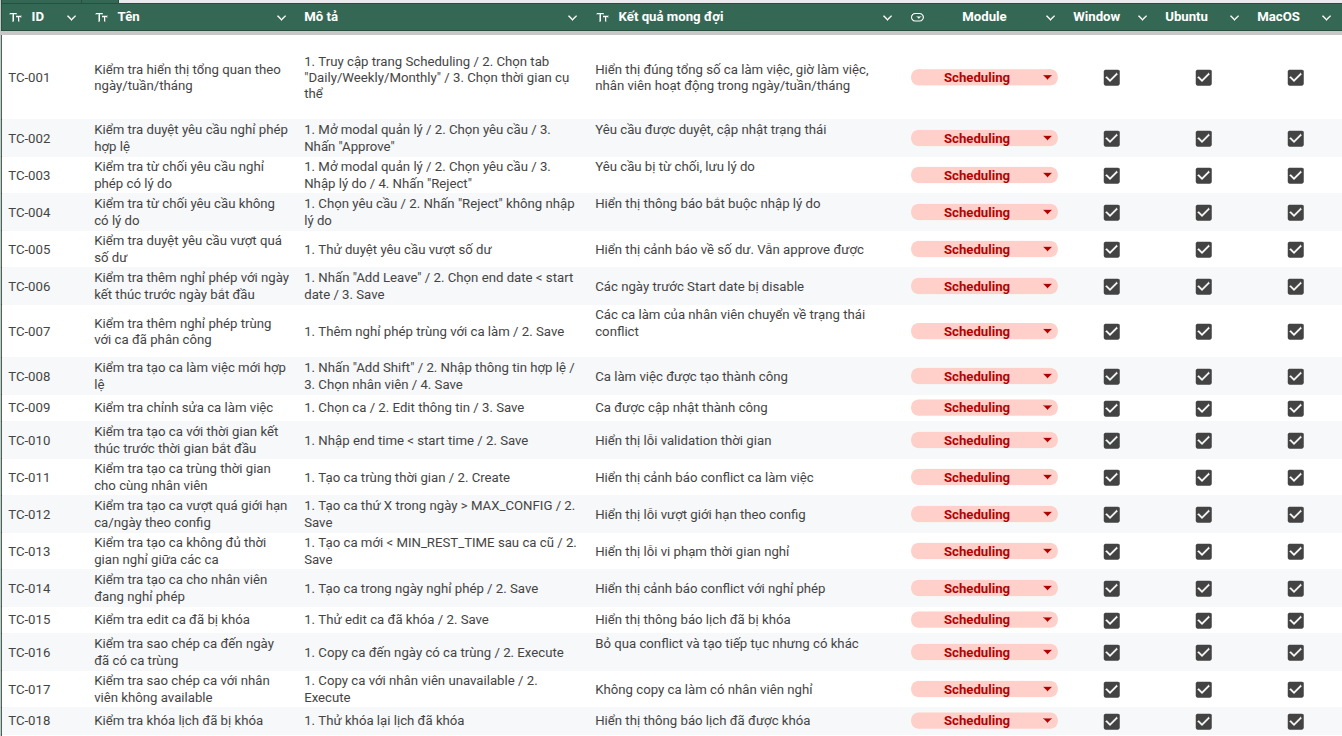
\includegraphics[width=14cm]{Images/hienthuc/test_schedule.png}
		\vspace{0.5cm}
        \caption{Kết quả kiểm thử Scheduling Module}
		\label{fig:schedule}
    \end{figure}
	Các test case (tạo/duyệt ca làm việc, nghỉ phép, kiểm tra trùng lặp, sao chép ca, khóa lịch) đều \textbf{Pass}.  
	Hệ thống cho kết quả chính xác trong các tình huống conflict, hỗ trợ quản lý nhân sự hiệu quả.
\end{itemize}

\subsubsection{Kết luận}
Kết quả kiểm thử cho thấy:  
\begin{itemize}
	\item \textbf{Booking, POS, Scheduling} hoạt động ổn định, tất cả test case đều \textbf{Pass}.  
	\item \textbf{Menu Module} còn tồn tại lỗi ở phần \textbf{Delete Category} và \textbf{Set Price Variant}, cần bổ sung sửa lỗi.  
\end{itemize}
Hệ thống đã chứng minh tính tương thích trên Windows, Ubuntu và MacOS. Tuy nhiên để tăng độ tin cậy, cần mở rộng thêm kiểm thử trên môi trường production (tích hợp dịch vụ email, thanh toán online, Cloudinary upload), vì kiểm thử hiện tại mới chạy trên \texttt{localhost}.
